\documentclass[12pt]{article}
\usepackage{amsthm,amssymb,amsmath,amsfonts}
\usepackage[a4paper, top=25mm, bottom=30mm, left=25mm, right=25mm]{geometry}
\usepackage[pagebackref=false,colorlinks,linkcolor=black,citecolor=black]{hyperref}
\usepackage[nameinlink]{cleveref}
 \AtBeginDocument{%
    \crefname{equation}{برابری}{equations}%
    \crefname{chapter}{فصل}{chapters}%
    \crefname{section}{بخش}{sections}%
    \crefname{appendix}{پیوست}{appendices}%
    \crefname{enumi}{مورد}{items}%
    \crefname{footnote}{زیرنویس}{footnotes}%
    \crefname{figure}{شکل}{figures}%
    \crefname{table}{جدول}{tables}%
    \crefname{theorem}{قضیه}{theorems}%
    \crefname{lemma}{لم}{lemmas}%
    \crefname{corollary}{نتیجه}{corollaries}%
    \crefname{proposition}{گزاره}{propositions}%
    \crefname{definition}{تعریف}{definitions}%
    \crefname{result}{نتیجه}{results}%
    \crefname{example}{مثال}{examples}%
    \crefname{remark}{نکته}{remarks}%
    \crefname{note}{یادداشت}{notes}%
    \crefname{observation}{مشاهده}{observations}%
    \crefname{algorithm}{الگوریتم}{algorithms}%
    \crefname{cproof}{برهان}{cproofs}%
}

\usepackage{tikz}
\usepackage{graphicx}
\usepackage{booktabs}
\usepackage{color}
\usepackage{graphicx}
\usepackage{subcaption}

\usepackage{setspace}
\doublespacing

\usepackage{titletoc}
\usepackage{tocloft}
\usepackage{enumitem}
\usepackage{amsmath, amssymb}
\usepackage{algorithm}
\usepackage[noend]{algorithmic}
\renewcommand{\algorithmicrequire}{\textbf{Input:}}
\renewcommand{\algorithmicensure}{\textbf{Output:}}

\usepackage{tabularx}
\makeatletter
\newcommand{\multiline}[1]{%
  \begin{tabularx}{\dimexpr\linewidth-\ALG@thistlm}[t]{@{}X@{}}
    #1
  \end{tabularx}
}
\makeatother

\usepackage{float}
\usepackage{verbatim}
\makeindex
\usepackage{sectsty}
\usepackage{xepersian}
\SepMark{-}
\settextfont[Scale=1.2,Path=fonts/,BoldFont=B Nazanin Bold.ttf]{B Nazanin.ttf}
\setlatintextfont{Times New Roman}
\renewcommand{\labelitemi}{$\bullet$}

\theoremstyle{definition}
\newtheorem{definition}{تعریف}[section]
\newtheorem{remark}[definition]{نکته}
\newtheorem{note}[definition]{یادداشت}
\newtheorem{example}[definition]{نمونه}
\newtheorem{question}[definition]{سوال}
\newtheorem{remember}[definition]{یاداوری}
\newtheorem{observation}[definition]{مشاهده}
\theoremstyle{theorem}
\newtheorem{theorem}[definition]{قضیه}
\newtheorem{lemma}[definition]{لم}
\newtheorem{proposition}[definition]{گزاره}
\newtheorem{corollary}[definition]{نتیجه}
\newtheorem*{cproof}{برهان}




\begin{document}
\fontsize{12pt}{14pt}\selectfont

\begin{minipage}{0.1\textwidth}

\includegraphics[width=3cm]{etc/IUST}
\end{minipage}%
\hfill%
\begin{minipage}{0.6\textwidth}\centering
\fontsize{13pt}{13pt}\selectfont
به‌ نام خدا \\
\textbf{درس یادگیری عمیق} \\
\textbf{تمرین سری ششم}\\
استاد درس : دکتر محمدرضا محمدی \\
دستیاران :  مهدی خورشا، سید محمد موسوی،\\ امیرحسین نمازی
\\
\vspace{0.25cm}
\begingroup
\fontsize{11pt}{11pt}\selectfont
دانشگاه علم و صنعت ایران، دانشکده مهندسی کامپیوتر \\
نیمسال دوم تحصیلی 1403 - 1404 \\
\endgroup
\end{minipage}%
\hfill%
\begin{minipage}{0.1\textwidth}

\end{minipage}

\vspace{0.5cm}

\noindent\rule{\textwidth}{1pt}

\centering {\fontsize{18}{22}\selectfont \textbf{مهلت تحویل : 1404/03/20 }}\\
{\fontsize{14}{22}\selectfont \textbf{لطفا به نکات موجود در سند قوانین انجام و تحویل تمرین ها دقت فرمایید. }}

\begin{enumerate}

    \section*{سوالات تئوری}
    \item 
\includegraphics[width=1cm]{figs/Forbidden_AI.jpg}
    در این درس با \href{https://arxiv.org/pdf/2006.11239}{مدل های انتشار نویز زدایی}\LTRfootnote{DDPM} آشنا شدید.\\
    اکنون \href{https://arxiv.org/pdf/2006.09011}{مدل های‌امتیازی شرطی‌شده با نویز}\LTRfootnote{NCSN} را مطالعه کرده و به پرسش‌های زیر پاسخ دهید(۱۵ نمره):
    
    \begin{enumerate}
        \item روش را کوتاه توضیح داده و بگویید \lr{Langevin dynamics} چیست و چه کارکردی در آن دارد؟
        \textcolor{blue}{
        \lr{Langevin dynamics} یک روش تکراری الهام گرفته شده از فیزیک است که می‌تواند برای نمونه‌برداری از داده‌ها استفاده شود. درواقع می‌تواند نمونه‌هایی را از توزیع \lr{p(x)} تنها با استفاده از تابع امتیاز تولید کند. برای هر توزیع احتمالی \lr{p(x)} ما گرادیان آن یعنی $\nabla_x \log p(x)$
         را خواهیم داشت (لگاریتم برای سهولت در محاسبات است) که ما آن را \lr{score function} می‌نامیم. علت اصلی این کار این است که در بسیاری از موارد، مدل کردن و تخمین \lr{score function} بسیار ساده‌تر از محاسبه توزیع احتمالی اصلی خواهد بود. در این روش با استفاده از یک انداره گام $\alpha > 0
        $ و تعداد تکرار مشخص $T$ و یک نمونه اولیه $x_0$ از فرمول زیر به دست می‌آید (دقت شود که $x_0$ می‌تواند یک نویز با توزیع نرمال باشد یا توزیع‌های پیشین در هر مرحله‌ای).
        $$
        x_t \leftarrow x_{t-1} + \alpha \nabla_x \log p(x_{t-1}) + \sqrt{2\alpha}\, z_t, \quad 1 \leq t \leq T
        $$
        نویز $z_t \sim \mathcal{N}(0, I)$ به منظور جلوگیری از حداقل‌های محلی اضافه شده است. بنابراین، یک مدل مولد می‌تواند پس از تخمین امتیاز با استفاده از یک شبکه عصبی $s_\theta(x) \approx \nabla_x \log p(x)$ از روش فوق برای نمونه‌برداری از $p(x)$ استفاده کند.\\        
        \textbf{روش مقاله}\\
        این مقاله ۵ تکنیک مهم را بیان می‌کند که در ادامه به توضیح هر یک از آن‌ها می‌پردازیم.
        مقیاس نویز اولیه که آن را $\sigma_1$ می‌نامیم، تا حد زیادی تنوع نمونه‌های نهایی را کنترل می‌کند. برای افزایش تنوع نمونه، ممکن است بخواهیم $\sigma_1$ را تا حد امکان بزرگ انتخاب کنیم. با این حال، اگر $\sigma_1$ بیش از حد بزرگ باشد به مقیاس‌های نویز بیشتری نیاز دارد (که در ادامه مورد بحث قرار خواهد گرفت) و این امر هزینه و زمان زیادی خواهد گرفت. برای همین ما به دنبال مقیاس نویز اولیه‌ای هستیم که این مورد را به خوبی کنترل کند.
        توزیع داده‌های دنیای واقعی پیچیده و تحلیل آنها دشوار است، بنابراین ما تلاش می‌کنیم تقریبی از آن به دست آوریم. فرض کنید یک دیتاست به صورت $\{ x^{(1)}, x^{(2)}, \dots, x^{(N)} \}$
        داریم که هر داده از آن از توزیع $p_{\text{\lr{data}}}(x)$ می‌آید. با فرض این که $N$ به مقدار کافی بزرگ باشد، توزیع دیتاست تقریبا برابر میانگین توزیع نمونه‌ها خواهد بود. یعنی:
        $$
        p_{\text{\lr{data}}}(x) \approx \hat{p}_{\text{\lr{data}}}(x) \triangleq \frac{1}{N} \sum_{i=1}^{N} \delta\big(x = x^{(i)}\big)
        $$
        حال اگر داده‌ها توسط یک توزیع نرمال با میانگین صفر و واریانس $\sigma_1^2 I$ یعنی 
        $\mathcal{N}(0, \sigma_1^2 I)$ 
        نویزی شود، توزیع تقریبی ما برابر خواهد بود با:
        $$
        p_{\sigma_1}(x) \triangleq \frac{1}{N} \sum_{i=1}^{N} p^{(i)}(x)
        $$
        که در آن مقدار $x$ تحت یک توزیع نرمال با میانگین $x^{(i)}$ و واریانس $\sigma_1^2 I$ خواهد بود. یعنی:
        $$
        p^{(i)}(x) \triangleq \mathcal{N}(x \mid x^{(i)}, \sigma_1^2 I)
        $$
        ما انتظار داریم که \lr{Langevin dynamics} هر توزیع $p^{(i)}(x)$ را با شروع از هر $p^{(j)}(x)$ در حالی که $i \neq j$ تخمین بزند.  
        حال با فرمول‌های گفته شده، یک $r^{(i)}(x)$ داریم که برابر است با احتمال این که نقطه $x$ از توزیع $i$ام آمده باشد. یعنی:
        $$
        r^{(i)}(x) \triangleq \frac{p^{(i)}(x)}{\sum_{k=1}^{N} p^{(k)}(x)}
        $$
        پس طبق فرمول بالا، تابع امتیاز برابر خواهد بود با:
        $$
        \hat{p}_{\sigma_1}(x) = \frac{1}{N} \sum_{i=1}^{N} p^{(i)}(x)
        $$
        $$
        \nabla_x \log \hat{p}_{\sigma_1}(x) 
        = \frac{\nabla_x \hat{p}_{\sigma_1}(x)}{\hat{p}_{\sigma_1}(x)} 
        = \frac{1}{\hat{p}_{\sigma_1}(x)} \cdot \frac{1}{N} \sum_{i=1}^{N} \nabla_x p^{(i)}(x)
        $$
        $$
        \nabla_x \log p^{(i)}(x) = \frac{\nabla_x p^{(i)}(x)}{p^{(i)}(x)}
        \;\;\;\;\;\;\Rightarrow\;\;\;\;\;\;
        \nabla_x p^{(i)}(x) = \nabla_x \log p^{(i)}(x) \cdot p^{(i)}(x)
        $$
        $$
        \nabla_x \log \hat{p}_{\sigma_1}(x) 
        = \frac{1}{\frac{1}{N} \sum_{k=1}^{N} p^{(k)}(x)} \cdot \frac{1}{N} \sum_{i=1}^{N} \nabla_x \log p^{(i)}(x) \, p^{(i)}(x)
        $$
        $$
        = \sum_{i=1}^{N} \nabla_x \log p^{(i)}(x) \cdot \frac{p^{(i)}(x)}{\sum_{k=1}^{N} p^{(k)}(x)}
        = \sum_{i=1}^{N} r^{(i)}(x) \, \nabla_x \log p^{(i)}(x)
        $$
        با فرض این که $x \in \mathbb{R}^D$ باشد، خواهیم داشت:
        $$
        \mathbb{E}_{p^{(i)}(x)} [r^{(j)}(x)] 
        = \int \frac{p^{(i)}(x) \, p^{(j)}(x)}{\sum_{k=1}^{N} p^{(k)}(x)} \, dx 
        \;\;\leq\;\;
        \int \frac{p^{(i)}(x) \, p^{(j)}(x)}{p^{(i)}(x) + p^{(j)}(x)} \, dx
        $$
        که با ساده‌سازی آن (صفحه 12 مقاله) به فرمول زیر دست خواهیم یافت:
        $$
        \mathbb{E}_{p^{(i)}(x)} [r^{(j)}(x)] \leq \tfrac{1}{2} \exp\!\left(-\frac{\lVert x^{(i)} - x^{(j)} \rVert_2^2}{8 \sigma_1^2}\right)
        $$
        برای این که از توزیع $p^{(j)}(x)$ به $p^{(i)}(x)$ برسیم ($i \neq j$)، باید 
        $\mathbb{E}_{p^{(i)}(x)} [r^{(j)}(x)]$ 
        بزرگ باشد، زیرا در غیر این صورت، گرادیان یعنی $\nabla_x \log \hat{p}_{\sigma_1}(x) 
        = \sum_{i=1}^{N} r^{(i)}(x) \, \nabla_x \log p^{(i)}(x)$
        مقدار $p^{(j)}(x)$ را نادیده می‌گیرد (در بخش ب بیشتر توضیح داده خواهد شد).  
        فرمول بالا به ما این را می‌گوید که 
        $\mathbb{E}_{p^{(i)}(x)} [r^{(j)}(x)]$ 
        زمانی که $\sigma_1$ نسبت به $\lVert x^{(i)} - x^{(j)} \rVert_2$ کوچک باشد، می‌تواند به صورت تصاعدی کاهش یابد.  
        در نتیجه، لازم است که $\sigma_1$ از نظر عددی با حداکثر فواصل جفت به جفت داده‌ها قابل مقایسه باشد.\\
        \textbf{تکنیک شماره ۱}\\
        $\sigma_1$ را به اندازه حداکثر فاصله اقلیدسی بین همه جفت داده آموزشی انتخاب کنید.  
        حال ما به انتخاب تعداد مقیاس نویز و میزان سطح نویز می‌پردازیم. زیرا همان‌گونه که بیان شد، ما نیاز به گرادیان‌های قابل اعتماد برای رسیدن به توزیع احتمالی مطلوب داریم. برای سادگی فرض می‌کنیم که در دیتاست تنها یک داده داریم.  
        ما توزیع داده نویزی را یک ابر کروی گوسی در نظر می‌گیریم که در آن $r$ و $\varphi$ به ترتیب مختصات شعاعی و زاویه‌ای $x$ را نشان می‌دهند. پس خواهیم داشت:
        این فرمول در واقع \lr{pdf} مربع کای (\lr{Chi-squared}) است که با اثبات (صفحه ۱۲ مقاله) خواهیم داشت:
        $$
        r - \sqrt{D}\,\sigma \;\;\xrightarrow{d}\;\; \mathcal{N}(0, \tfrac{\sigma^2}{2}) \quad \text{\lr{when } } \text{\lr{D}} \to \infty
        $$
        پس خواهیم داشت:
        $$
        p(r) \approx \mathcal{N}\big(r \mid \sqrt{D}\,\sigma, \tfrac{\sigma^2}{2}\big)
        $$
        همچنین برای ساده‌سازی، یک تغییر متغیر خواهیم داشت که در آن:
        $$
        m_i \triangleq \sqrt{D}\,\sigma, \quad s_i^2 \triangleq \tfrac{\sigma^2}{2}
        $$
        پس:
        $$
        p_{\sigma_i}(r) = \mathcal{N}(r \mid m_i, s_i^2)
        $$
        هدف اصلی ما این است که $p_{\sigma_i}(x)$ به اندازه کافی با مناطق $p_{\sigma_{i-1}}(x)$ همپوشانی داشته باشد، زیرا به گرادیان آن نیاز داریم که به $p_{\sigma_i}(x)$ برسیم.  
        همچنین، همان‌گونه که گفته شد، جز زاویه‌ای (\lr{angular component}) یعنی $p(\varphi)$ بین تمام مقیاس‌های نویز مشترک است چون $p_{\sigma_i}(x)$ یک \lr{isotropic Gaussian} است. بنابراین تنها نیاز داریم تا جز شعاعی (\lr{radial component}) دارای همپوشانی باشد.
        \begin{figure}[h]
            \centering
            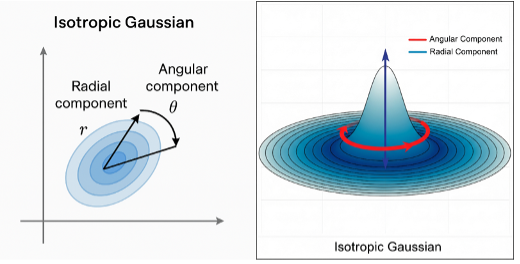
\includegraphics[width=\textwidth]{figs/Q1_1.png}
            \caption{جز شعاعی و زاویه‌ای در توزیع گوسی}
            \label{fig:q1_1}  
        \end{figure}
        حال بر اساس قانون سه سیگما (\lr{Three-sigma rule}) که در تصویر ۲ مشاهده می‌کنید، 
        $p_{\sigma_{i-1}}(x)$ 
        دارای تراکم بالایی در بازه زیر خواهد بود: 
        $$
        [m_{i-1} - 3s_{i-1}, \; m_{i-1} + 3s_{i-1}]
        $$
        \begin{figure}[h]
            \centering
            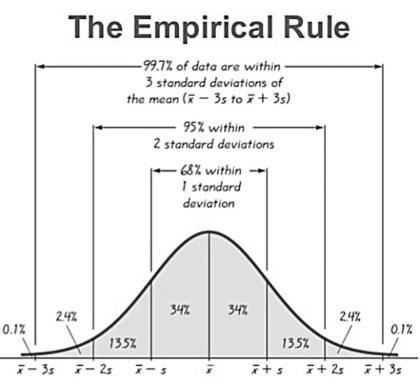
\includegraphics[width=\textwidth]{figs/Q1_2.jpg}
            \caption{\lr{Three-sigma rule}}
            \label{fig:q1_2}  
        \end{figure}
        اکنون یک مرور از چیزهایی که گفتیم و سپس نتیجه‌گیری نهایی:\\
        1)
        $$
        p_{\sigma_i}(r) = \mathcal{N}(r \mid m_i, s_i^2), 
        \quad m_i \triangleq \sqrt{D}\,\sigma, 
        \quad s_i^2 \triangleq \tfrac{\sigma^2}{2}
        $$
        2)
        $$
        m_{i-1} = \sqrt{D}\,\sigma_{i-1} = \sqrt{D}\,\gamma\sigma_i = \gamma m_i,
        \quad \gamma = \frac{\sigma_{i-1}}{\sigma_i}
        $$
        3)
        $$
        s_{i-1}^2 = \tfrac{\sigma_{i-1}^2}{2} 
        \;\;\;\Rightarrow\;\;\;
        s_{i-1} = \frac{\sigma_{i-1}}{\sqrt{2}} = \frac{\gamma\sigma_i}{\sqrt{2}} = \gamma s_i
        $$
        4)
        $$
        I_{i-1} = [\, m_{i-1} - 3s_{i-1}, \; m_{i-1} + 3s_{i-1} \,]
        $$
        5)از معادله (۱):
        $$
        z = \frac{r - m_i}{s_i} \quad \Rightarrow \quad r = z s_i + m_i
        $$
        6)با استفاده از معادلات (۲)، (۳)، (۴)، (۵) خواهیم داشت:
        $$
        z \in \left[ \frac{\gamma m_i - 3\gamma s_i - m_i}{s_i}, \; \frac{\gamma m_i + 3\gamma s_i - m_i}{s_i} \right]
        $$
        \paragraph{\lr{Lower Bound}}
        $$
        \frac{\gamma m_i - 3\gamma s_i - m_i}{s_i} 
        = \frac{m_i(\gamma - 1)}{s_i} - 3\gamma
        = \frac{\sqrt{D}\,\sigma_i (\gamma - 1)}{\sigma_i/\sqrt{2}} - 3\gamma
        = \sqrt{2D}(\gamma - 1) - 3\gamma
        $$
        \paragraph{\lr{Upper Bound}}
        $$
        \frac{\gamma m_i + 3\gamma s_i - m_i}{s_i} 
        = \sqrt{2D}(\gamma - 1) + 3\gamma
        $$
        پس در نتیجه خواهیم داشت:
        $$
        p_{\sigma_i}\big(r \in I_{i-1}\big) 
        = \Phi\big(\sqrt{2D}(\gamma - 1) + 3\gamma\big) 
        - \Phi\big(\sqrt{2D}(\gamma - 1) - 3\gamma\big) 
        = C
        $$
        در فرمول بالا $\Phi$ به معنای \lr{CDF} توزیع نرمال استاندارد است.  
        این فرمول بیان می‌کند که چه مقدار از جرم توزیع $p_{\sigma_i}(x)$ داخل بازه‌ای قرار می‌گیرد که برای $p_{\sigma_{i-1}}(x)$ پرتراکم‌ترین ناحیه است (در واقع همان $99/7$ درصد در تصویر ۲). 
        نکته مهم در فرمول بالا $\gamma$ است که تنها به نسبت بین دو نویز وابسته است (نه به خود نویزها). این امر به ما اجازه می‌دهد که به‌صورت عددی مقدار بهینه‌ی $\gamma$ را پیدا کنیم تا مقدار همپوشانی برابر $C$ باشد.  
        در حالت ایده‌آل باید $C=1$ باشد، اما تعداد زیاد $L$ هزینه نمونه‌برداری را بسیار افزایش می‌دهد.  
        برای همین مقاله پیشنهاد می‌کند که $C = 0.5$ در نظر گرفته شود.\\
        \textbf{تکنیک شماره 2:$\{\sigma_i\}_{i=1}^{L}$  را بر اساس معادله گفته شده و با  $C \approx 0.5$  محاسبه کنید.}\\
        طبق تکنیک 1 و 2، برای تصاویر با وضوح بالا، نیاز به نویز اولیه بزرگ و تعداد زیادی مقیاس نویز داریم. در روش اصلی مدل \lr{NCSN}، برای هر مقدار نویز $\sigma$، یک مجموعه پارامتر جدید در لایه‌های نرمال‌سازی شبکه تعریف می‌شود. این روش دو مشکل دارد: مصرف زیاد حافظه و وابستگی به لایه نرمال‌سازی (اگر معماری شبکه نرمال‌سازی نداشته باشد، این روش قابل استفاده نیست).  
        پس به‌جای شبکه‌ای که به $\sigma$ وابسته باشد، از یک شبکه ساده استفاده می‌کنیم که به $\sigma$ وابسته نیست.  
        از نظر تئوری، تابع امتیاز واقعی توزیع $N(x \mid 0, \sigma^2/2)$ دارای نرم متوسطی متناسب با $\sqrt{D}/\sigma$ است. مشاهدات تجربی هم نشان داده‌اند که نرم شبکه آموزش‌دیده تقریباً با $1/\sigma$ متناسب است. بنابراین، به‌جای شبکه‌ای که به $\sigma$ وابسته باشد، از یک شبکه ساده استفاده می‌کنیم که به $\sigma$ وابسته نیست و فقط خروجی آن در $1/\sigma$ ضرب می‌شود.\\  
        \textbf{تکنیک 3: تابع امتیاز وابسته به نویز به‌صورت زیر تعریف می‌شود:}\\
        $$
        \frac{s_\theta(x)}{\sigma} = s_\theta(x, \sigma)
        $$
        در این تکنیک ما به تعداد مراحل نمونه‌برداری به ازای هر مقیاس نویز ($T$) و اندازه گام ($\varepsilon$) را مشخص خواهیم کرد. توجه کنید که در الگوریتم 1، ما الگوریتم \lr{Langevin dynamics} را به ازای مقیاس نویزهای مختلف، $T$ بار اجرا می‌کنیم و در هر بار تکرار این حلقه، گرادیان را ضرب در $\frac{\varepsilon \, \sigma_i^2}{\sigma_L^2}$
        می‌کنیم.
        \begin{figure}[h]
            \centering
            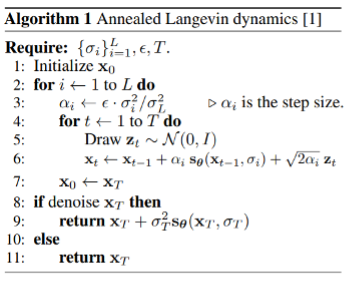
\includegraphics[width=\textwidth]{figs/Q1_3.png}
            % \caption{\lr{Three-sigma rule}}
            \label{fig:q1_3}  
        \end{figure}
        باتوجه به اثبات صفحه 13 خواهیم داشت:
        $$
        \frac{s_T^2}{\sigma_i^2}=\left(1-\frac{\epsilon}{\sigma_L^2}\right)^{2 T}\left(\gamma^2-\frac{2 \epsilon}{\sigma_L^2-\sigma_L^2\left(1-\frac{\epsilon}{\sigma_L^2}\right)^2}\right)+\frac{2 \epsilon}{\sigma_L^2-\sigma_L^2\left(1-\frac{\epsilon}{\sigma_L^2}\right)^2} .
        $$
        در فرمول بالا، $s_T^2$ در واقع واریانس داده‌های ما پس از $T$ بار اجرای حلقه دوم در الگوریتم 1 است. طبیعی است که ما دوست داریم این مقدار در هر مقیاس نویز، به طور تقریبی از توزیع  $N(x \mid 0, \sigma_i^2 I)$ 
        پیروی کند. یعنی مقدار فرمول بالا برای تمام مقیاس‌های نویز برابر 1 باشد؛ ولی شوربختانه این کار نیاز به یک $T$ بسیار بزرگ دارد که هزینه زیادی خواهد داشت. برای همین، مقاله پیشنهاد می‌کند که ابتدا $T$ را براساس بودجه محاسباتی خود مشخص کنیم و سپس با فرمول بالا $\varepsilon$ را بر مبنای $T$ پیدا کنیم.\\
        \textbf{تکنیک 4: $T$ را تا جایی که بودجه محاسباتی اجازه می‌دهد بزرگ انتخاب کنید و سپس مقداری را انتخاب کنید که معادله بالا را به 1 نزدیک کند.}\\
        اگرچه در \lr{NCSN} ها، مقدار \lr{loss} در طول آموزش کاهش پیدا می‌کند، ولی گاهی مشاهده می‌کنیم که نمونه‌های تصویر تولید شده، کیفیت بصری خوبی ندارند. به تصویر زیر توجه کنید:
        \begin{figure}[h]
            \centering
            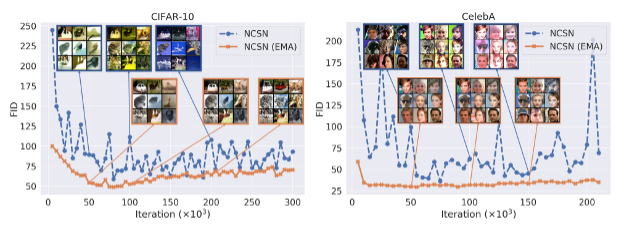
\includegraphics[width=\textwidth]{figs/Q1_4.png}
            \caption{\lr{FIDs and color artifacts over the course of training}}
            \label{fig:q1_4}  
        \end{figure}
        مشاهده می‌شود که \lr{NCSN} اغلب در طول آموزش، نوسانات زیادی دارد و همچنین تصاویر مصنوعی تولید می‌کند. این مشکل را می‌توان به راحتی با میانگین متحرک نمایی (\lr{EMA}) حل کرد. یعنی:
        $$
        \theta' \gets m \, \theta' + (1-m) \, \theta_i
        $$
        در فرمول بالا، $m$ پارامتر \lr{momentum} است و معمولاً برابر $0.999$ می‌باشد. این روش تضمین می‌کند که تخمین‌ها پایدارتر باشند. ما به جای $s_{\theta_i}(x, \sigma)$ از $s_{\theta'}(x, \sigma)$ استفاده می‌کنیم.
        \textbf{تکنیک 5:\lr{EMA} را برای پارامترها اعمال کنید.}\\
        }
        \item چگونه مدل‌های انتشار چالش فرض چندگانه و چگالی داده کم را برطرف می‌کنند؟
        \textcolor{blue}{
        اولین مشکل این روش، فرض چندگانه  است. فرضیه چندگانه بیان می‌کند که داده‌های با ابعاد بالا در دنیای واقعی بر روی فضا با بعد کمتر می‌توانند قرار گیرند. این فرضیه به طور تجربی برای بسیاری از مجموعه‌داده‌ها صادق است. تحت فرضیه چندگانه، مدل‌های مولد مبتنی بر امتیاز با مشکل کلیدی مواجه خواهند شد. ازآنجایی‌که تابع امتیاز یک گرادیان است که در فضای محیطی گرفته شده است، زمانی که \lr{x} به ابعاد کم محدود شود، این گرادیان تعریف نشده است (تصویر4).\\
        \begin{figure}[h]
            \centering
            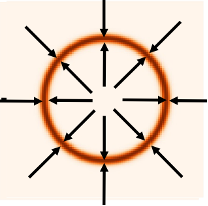
\includegraphics[width=\textwidth]{figs/Q1_2_1.png}
            \caption{فرض چندگانه}
            \label{fig:q1_2_1}  
        \end{figure}
        برای برطرف‌کردن این مشکل باید مقداری نویز به داده¬ها اضافه کنیم. تأثیر منفی فرض چندگانه بر تخمین امتیاز را می‌توان به‌وضوح در تصویر (5) مشاهده کرد. جایی که یک شبکه \lr{ResNet} برای تخمین امتیاز داده ها در \lr{CIFAR-10} آموزش داده¬شده¬است. همان¬طور که سمت چپ تصویر (5) نشان می دهد، هنگامی که این شبکه بر روی تصاویر اصلی \lr{CIFAR-10} آموزش داده می شود، خطا ابتدا کاهش می یابد و سپس به طور نامنظم در نوسان است. در مقابل، اگر به داده¬ها مقدار اندکی نویز گاوسی اضافه کنیم منحنی خطا همگرا می¬شود (سمت راست تصویر 4).
        \begin{figure}[h]
            \centering
            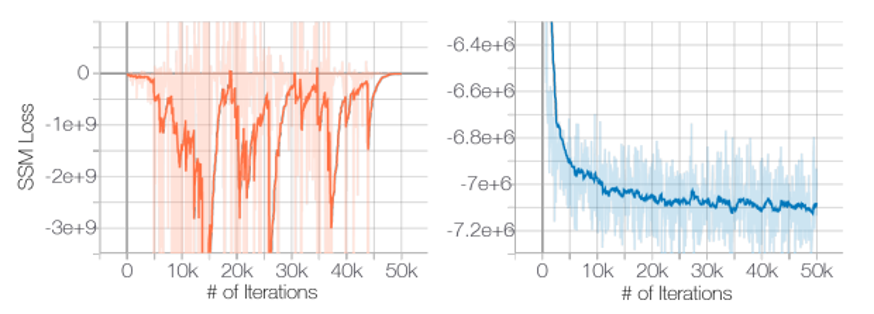
\includegraphics[width=\textwidth]{figs/Q1_2_2.png}
            \caption{مقایسه مقدار ضرر در دو حالت داده بدون نویز و با نویز گوسی اندک}
            \label{fig:q1_2_2}  
        \end{figure}
        مشکل دوم مناطق با تراکم داده کم  است. در مناطق با تراکم داده کم\LTRfootnote{low data density regions}، تطبیق امتیاز ممکن است به دلیل فقدان نمونه داده، شواهد کافی برای تخمین دقیق عملکردهای امتیاز نداشته باشد. هنگام نمونه‌گیری با \lr{Langevin dynamics} و زمانی که داده‌ها در فضای با ابعاد بالا قرار دارند، نمونه اولیه ما در مناطق با تراکم پایین بسیار محتمل است؛ بنابراین، داشتن یک مدل مبتنی بر امتیاز نادرست، \lr{Langevin dynamics} را از همان ابتدای روش از مسیر خارج می‌کند و از تولید نمونه‌های باکیفیت بالا که نماینده داده‌ها هستند، جلوگیری می‌کند.
        \begin{figure}[h]
            \centering
            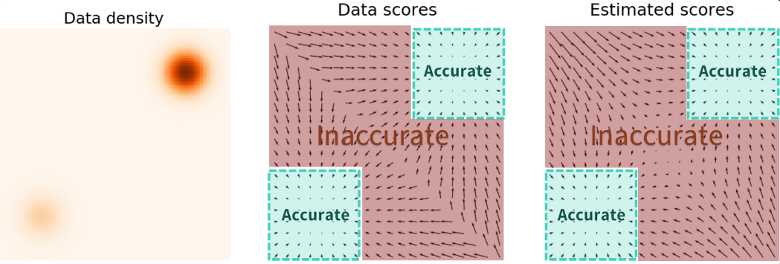
\includegraphics[width=\textwidth]{figs/Q1_2_3.png}
            \caption{امتیازات تقریبی تنها در مناطق پرتراکم دقیق هستند}
            \label{fig:q1_2_3}  
        \end{figure}
        اما چگونه می‌توانیم از دشواری تخمین امتیاز دقیق در مناطق با تراکم داده کم عبور کنیم؟ راه‌حل این است که همانند مشکل اول، نقاط داده را نویزی کنیم و مدل‌های مبتنی بر امتیاز را روی نقاط داده پر نویز آموزش دهیم.
        هنگامی که بزرگی نویز به‌اندازه کافی بزرگ باشد، می‌تواند مناطق کم‌تراکم داده را پر کند تا دقت امتیازهای تخمینی را بهبود بخشد.
        \begin{figure}[h]
            \centering
            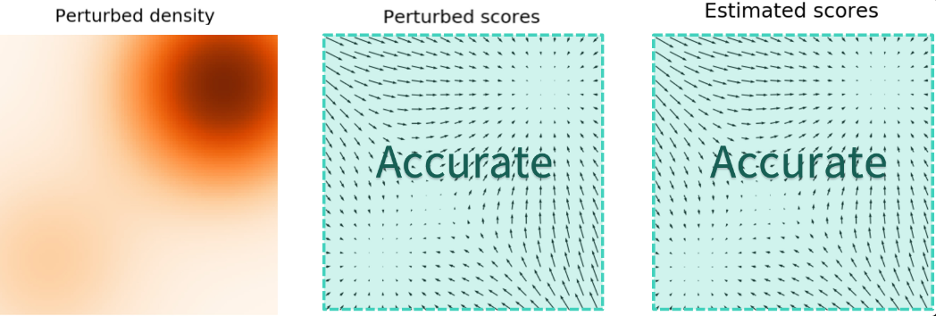
\includegraphics[width=\textwidth]{figs/Q1_2_4.png}
            \caption{امتیازات تخمینی دقیق در همه جا به دلیل افزودن نویز}
            \label{fig:q1_2_4}  
        \end{figure}
        اما این تراکم داده کم سبب ایجاد مشکلی دیگر نیز می‌شود. هنگامی که دو حالت توزیع داده توسط مناطق با چگالی کم از هم جدا می‌شوند، \lr{Langevin dynamics} نمی‌تواند وزن‌های مرتبط به این دو حالت را به‌درستی کشف کند و بنابراین ممکن است به توزیع واقعی همگرا نشوند.  
        به‌عنوان‌مثال توزیع $p_{\text{\lr{data}}}(x)$ را در نظر بگیرید که در آن $p_1(x)$ و $p_2(x)$ توزیع‌های ازهم‌گسسته هستند و $\pi \in (0,1)$. آنگاه خواهیم داشت:
        $$
        p_{\text{data}}(x) = \pi p_1(x) + (1-\pi)p_2(x)
        $$
        $$
        p_{\text{data}}(x) =
        \begin{cases}
        \pi p_1(x), & x \in A\\
        (1-\pi) p_2(x), & x \in B
        \end{cases}, \quad A \cap B = \emptyset
        $$
        در این صورت تابع امتیاز به شکل زیر خواهد بود:
        $$
        \nabla_x \log p(x) =
        \begin{cases}
        \nabla_x [\log \pi + \log p_1(x)], & x \in A\\
        \nabla_x [\log (1-\pi) + \log p_2(x)], & x \in B
        \end{cases} =
        \begin{cases}
        \nabla_x \log p_1(x), & x \in A\\
        \nabla_x \log p_2(x), & x \in B
        \end{cases}
        $$
        که مشاهده می‌شود تابع امتیاز اصلاً به $\pi$ وابستگی ندارد و ازآنجایی‌که \lr{Langevin dynamics} برای نمونه‌برداری از تابع امتیاز استفاده می‌کند، نمونه‌های به‌دست‌آمده به $\pi$ بستگی ندارند.\\  
        برای حل این مسئله، ابتدا به رویکردی که برای دو مشکل قبلی ارائه شده بود، نگاهی بیندازیم. در موارد پیشین، با افزودن نویز به داده‌ها مسئله را بهبود بخشیدیم، اما سؤال اساسی اینجا این است که چگونه می‌توانیم به طور معقول میزان و مقیاس نویز را انتخاب کنیم تا بهترین نتایج را بگیریم.\\ 
        نویز بزرگ‌تر بدیهی است که می‌تواند مناطق کم‌تراکم بیشتری را برای تخمین امتیاز بهتر پوشش دهد، اما داده‌ها را بیش از حد خراب می‌کند و آن را به طور قابل‌توجهی نسبت به توزیع اصلی تغییر می‌دهد. نویز کوچک‌تر، از سوی دیگر، باعث خرابی کمتری در توزیع داده‌های اصلی می‌شود، اما مناطق با چگالی کم را آن‌طور که می‌خواهیم پوشش نمی‌دهد. به همین منظور ما از روشی به نام \lr{annealed Langevin dynamics} استفاده می‌کنیم.  
        ایده \lr{annealed Langevin dynamics} این است که نویز را به‌صورت مرحله‌به‌مرحله اضافه کنیم. فرض کنید که ما از نویز گوسی و $L$ مقدار مختلف انحراف معیار استفاده می‌کنیم (توجه شود که میزان این نویزها در مقاله دوم و در تکنیک 1 و 2 مورد بحث قرار گرفت)، به‌طوری که:
        $$
        \sigma_1 < \sigma_2 < \dots < \sigma_L
        $$
        در ابتدا، ما با وضعیتی که داده‌ها به آن وارد می‌شوند و تحت تأثیر تمامی نویزهای گوسی قرار دارند، سعی داریم تا حالت اولیه داده‌ها را با این نویزها تخریب کنیم. سپس، تلاش می‌کنیم تا توزیع داده‌ها را تخمین بزنیم. این توزیع تا حدی به شکل یک توزیع نرمال نزدیک است و به دلیل این شباهت، ما بسیار سریع می‌توانیم به جواب موردنظرمان نزدیک شویم.\\
        بعد از آن، باتوجه‌به همگرایی سریعی که در مرحله پیشین به دست آورده‌ایم، از آن نقطه به بعد به ادامه کار می‌پردازیم. در واقع، با تحلیل داده‌ها به‌صورت تدریجی و مرحله‌به‌مرحله، ما به نقاط بهینه‌ای همگرا می‌شویم که این امر به ما کمک می‌کند که تخمین‌های ما از توزیع داده‌ها به‌دقت بهتری برسد. در نهایت، این رویکرد باعث می‌شود که تولید تصاویر برای ما آسان‌تر شود و به ما امکان می‌دهد تا بادقت بیشتری به تخمین توزیع داده‌ها برسیم (تصویر 8).
        \begin{figure}[h]
            \centering
            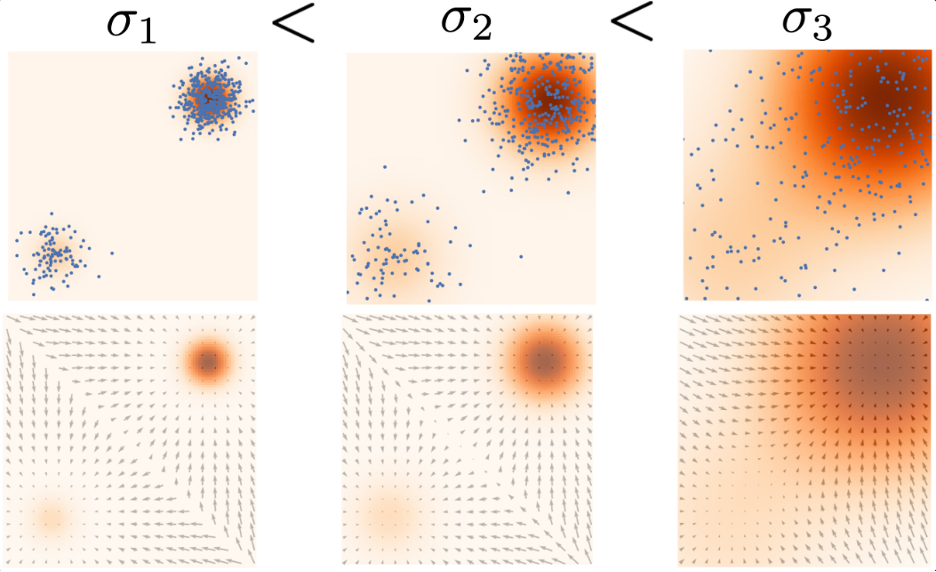
\includegraphics[width=\textwidth]{figs/Q1_2_5.png}
            \caption{\lr{annealed Langevin dynamics}}
            \label{fig:q1_2_5}  
        \end{figure}\\
        }
        \item اندازه نویز افزوده شده و گام زمانی چه تاثیری در مدل‌های انتشار دارد?برای مثال اگر به جای 40 مرحله نویز تنها 3 گام نویز ولی با اندازه بیشتری افزوده شود یا برعکس 80 گام نویز با اندازه کمتری افزوده شود، هر کدام چه برتری و کاستی‌هایی دارد؟
        
        \textcolor{blue}{
        مقیاس‌های نویز برای موفقیت \lr{NCSN} ها بسیار مهم هستند. شبکه‌های \lr{score base} که با یک نویز واحد آموزش دیده‌اند، هرگز نمی‌توانند نمونه‌های قانع‌کننده‌ای برای تصاویر بزرگ تولید کنند. به طور شهودی، نویز بالا تخمین توابع امتیاز را تسهیل می‌کند، اما منجر به نمونه‌های خراب نیز می‌شود؛ در حالی که نویز کمتر نمونه‌های تمیزی ارائه می‌دهد اما تخمین توابع امتیاز را دشوارتر می‌کند. بنابراین باید مقیاس‌های نویز مختلف را با هم به کار برد تا از هر دو حالت بهترین استفاده را برد. همچنین درباره تعداد گام زمانی، در تکنیک 2 گفته شد که اید به تعدادی باشد که مقیاس‌های نویز همپوشانی داشته باشند و اگر هم خیلی زیاد باشد، هزینه نمونه‌برداری را افزایش می‌دهد. 
        }
    \end{enumerate}

     
    \item 
\includegraphics[width=1cm]{figs/Forbidden_AI.jpg}
    
    \lr{WGAN}، که در این \href{https://arxiv.org/pdf/1701.07875}{مقاله} معرفی شد، یکی از اولین گام‌های بزرگ به سوی پایدارسازی آموزش \lr{GAN} بود. با چند تغییر، نویسندگان توانستند نشان دهند چگونه می‌توان \lr{GAN‌} هایی را آموزش داد که دارای دو ویژگی زیر باشند:
    
    \begin{itemize}
      \item یک معیار ضرر معنادار که با همگرایی \lr{generator} و کیفیت نمونه‌ها همبستگی دارد.
      \item بهبود پایداری فرآیند بهینه‌سازی. به طور خاص، این مقاله تابع ضرر واسرشتاین را برای هر دو \lr{discriminator} و \lr{generator} معرفی می‌کند. استفاده از این تابع ضرر به جای \lr{binary cross-entropy} منجر به همگرایی پایدارتر \lr{GAN} می‌شود.
    \end{itemize}
    
    در بسیاری از موارد، الگوریتم \lr{GAN} می‌تواند به عنوان کمینه‌سازی انحراف بین توزیع داده‌ها \( p_{\text{\lr{data}}} \) و توزیع مدل \( p_g \) در نظر گرفته شود. در این مسئله، ما یک مشکل با انحراف‌های مختلف (مثلاً انحراف \lr{Jensen-Shannon} و انحراف \lr{KL}) و یک راه‌حل بالقوه برای رفع آن (\lr{Wasserstein Distance}) را بررسی خواهیم کرد(۲۰ نمره).
    
    \begin{enumerate}
        \item[الف)] فرض کنید \( p_{\text{\lr{data}}} \sim \mathcal{N}(\theta_0, \epsilon^2) \) و \( p_g \sim \mathcal{N}(\theta, \epsilon^2) \) توزیع‌های نرمال با انحراف معیار \( \epsilon \) باشند که به ترتیب حول \( \theta_0 \in \mathbb{R} \) و \( \theta \in \mathbb{R} \) مرکزیت دارند. نشان دهید که:
        \[
        D_{\text{\lr{KL}}}(p_g \,\|\, p_{\text{\lr{data}}}) = \frac{(\theta - \theta_0)^2}{2\epsilon^2}
        \]

        \textcolor{blue}{
      $$
        \begin{aligned}
        \operatorname{KL}\left(p_\theta(x) \| p_{\text {data }}(x)\right) & =\mathbb{E}_{x \sim \mathcal{N}\left(\theta, \epsilon^2\right)}\left[\log \frac{\exp \left(-\frac{1}{2 \epsilon^2}(x-\theta)^2\right)}{\exp \left(-\frac{1}{2 \epsilon^2}\left(x-\theta_0\right)^2\right)}\right] \\
        & =\mathbb{E}_{x \sim \mathcal{N}\left(\theta, \epsilon^2\right)}\left[\frac{1}{2 \epsilon^2}\left(-(x-\theta)^2+\left(x-\theta_0\right)^2\right)\right] \\
        & =\mathbb{E}_{x \sim \mathcal{N}\left(\theta, \epsilon^2\right)}\left[\frac{1}{2 \epsilon^2}\left(2 x \theta-2 x \theta_0-\theta^2+\theta_0^2\right)\right] \\
        & =\frac{1}{2 \epsilon^2}\left(2 \theta^2-2 \theta \theta_0-\theta^2+\theta_0^2\right) \\
        & =\frac{\left(\theta-\theta_0\right)^2}{2 \epsilon^2} .
        \end{aligned}
    $$
      }
    
        \item[ب)] فرض کنید \( p_{\text{\lr{data}}} \) و \( p_g \) هر دو جرم احتمال را فقط در یک بخش بسیار کوچک از دامنه داشته باشند؛ یعنی، حد \( \epsilon \rightarrow 0 \). چه اتفاقی برای \( D_{\text{\lr{KL}}}(p_g \,\|\, p_{\text{\lr{data}}}) \) و مشتق آن نسبت به \( \theta \)، با فرض اینکه \( \theta \ne \theta_0 \)، می‌افتد؟
        
        \textcolor{blue}{
        مگر اینکه $\theta = \theta_0$ باشد، هم $\text{\lr{KL}}(p_\theta(x) \, \| \, p_{\text{\lr{data}}}(x))$ 
        و هم مشتق آن به سمت بی‌نهایت میل می‌کنند. اگر دیسکریمناتور به صورت بهینه آموزش داده شود، ژنراتور گرادیان‌های بسیار بزرگی دریافت خواهد کرد و در نتیجه آموزش ناپایدار خواهد بود.
        }
        \item[ج)] آیا این امر مشکلی برای یک \lr{GAN} که با تابع ضرر تعریف‌شده‌ی زیر آموزش داده شده‌ باشد، ایجاد می‌کند؟ چرا؟
        \[
        L_G(\theta; \phi) = \mathbb{E}_{x \sim p_\theta(x)}[\log(1 - D_\phi(x))] - \mathbb{E}_{x \sim p_\theta(x)}[\log D_\phi(x)]
        \]

        \textcolor{blue}{
        مگر اینکه $\theta = \theta_0$ باشد، $L_G$ می‌تواند با میل دادن $D_\phi(\theta)$ به $-\infty$ یا $D_\phi(\theta_0)$ به $\infty$ به سمت $-\infty$ میل کند. بنابراین، هیچ دیسکریمناتوری وجود ندارد که $L_D$ را کمینه کند.
        }
        \item[د)] تحت همان شرایط (ب)، انحراف \lr{KL}، انحراف \lr{JS} و فاصله واسرشتاین را مقایسه کنید.

        \textcolor{blue}{
        در حالت $\epsilon \to 0$ برای هر حالت داریم:  
        انحراف \lr{KL} به سمت $\infty$ و انحراف \lr{JS} به سمت $\log(2)$ میل می‌کنند، که در اولی گرادیان به شدت ناپایدار است و در دومی صفر است. ولی حتی اگر توزیع‌ها همپوشانی نداشته باشند، فاصله \lr{Wasserstein} مقدار محدودی دارد و گرادیان آن معنادار باقی می‌ماند. بنابراین پایدار و قابل یادگیری است. به همین دلیل، مقاله \lr{WGAN} تابع ضرر واسرشتاین را پیشنهاد می‌دهد تا این ناپایداری‌ها را رفع کند.
        }
    \end{enumerate}

    
    \item 
\includegraphics[width=1cm]{figs/Forbidden_AI.jpg}
    در ارتباط با \lr{DDPM} به سوالات زیر پاسخ دهید(۲۰ نمره):
    \begin{enumerate}
    \item فرض کنید $x_{t}$ متغیر تصادفی(یک نمونه داده مثلا یک تصویر)‌ای است که در فرایند \lr{Forward Diffusion Process} با اضافه شدن مقداری نویز به $x_{t-1}$ بدست می‌آید. بر این اساس عبارت زیر را توضیح دهید:
    $$
    x_t = \sqrt{1 - \beta_t} \, x_{t-1} + \sqrt{\beta_t} \, \epsilon
    $$

    \textcolor{blue}{
    این رابطه نشان‌دهنده‌ی مرحله‌ای از فرایند انتشار رو به جلو است. در این فرآیند، با شروع از تصویر اصلی $x_0$، به‌تدریج نویز گاوسی اضافه می‌شود تا داده به یک نویز کامل تبدیل شود.\\
    \textbf{تفسیر هر جزء از فرمول:}\\
    \begin{itemize}
        \item $x_t$ : این متغیر تصادفی، نشان‌دهنده داده (مثلاً تصویر) در گام فعلی ($t$) است. این تصویر ترکیبی از تصویر گام قبلی و نویز جدید اضافه شده است.
        \item $x_{t-1}$ : این متغیر تصادفی، داده در گام قبلی ($t-1$) را نشان می‌دهد. این همان تصویری است که قرار است در این گام به آن نویز اضافه شود.
        \item $\beta_t$ : این پارامتر یک مقدار کوچک و مثبت است که میزان نویزی را که در گام $t$ به تصویر اضافه می‌شود، تعیین می‌کند. این مقدار معمولاً در طول زمان از یک عدد کوچک (مانند $0.0001$) تا یک عدد بزرگتر (مانند $0.02$) به صورت خطی یا کوسینی افزایش می‌یابد. افزایش $\beta_t$ باعث می‌شود در گام‌های اولیه نویز کم و در گام‌های انتهایی نویز بیشتری اضافه شود.
        \item $\sqrt{1-\beta_t} \, x_{t-1}$ : این بخش، سهمی از تصویر اصلی گام قبلی $x_{t-1}$ است که حفظ شده و به گام جدید منتقل می‌شود. ضریب $\sqrt{1-\beta_t}$ نشان می‌دهد که چه مقدار از اطلاعات تصویر اصلی باقی می‌ماند و به گام بعدی منتقل می‌شود. هرچه $\beta_t$ بزرگ‌تر باشد، این ضریب کوچکتر شده و اطلاعات کمتری از تصویر قبلی حفظ می‌شود.
        \item $\sqrt{\beta_t} \, \epsilon$ : این بخش، همان نویزی است که در این مرحله به تصویر اضافه می‌شود. ضریب $\sqrt{\beta_t}$ میزان نویز اضافه شده را کنترل می‌کند. هرچه $\sqrt{\beta_t}$ بزرگ‌تر باشد، نویز بیشتری به تصویر اضافه می‌شود.
        \item $\epsilon \sim N(0,I)$ : این متغیر تصادفی، نویز جدیدی است که از یک توزیع نرمال (گوسی) استاندارد نمونه‌برداری می‌شود. این نویز دارای میانگین صفر و واریانس واحد است.
    \end{itemize}
    }
    \item با استفاده از ترفند تغییر پارامتر\LTRfootnote{Reparameterization trick} نشان دهید عبارت قسمت (آ) را می‌توان بصورت زیر نوشت:\\
    $$
    x_t = \sqrt{\bar{\alpha}_t} \, x_0 + \sqrt{1 - \bar{\alpha}_t} \, \epsilon
    $$

    \textcolor{blue}{
    \begin{figure}[ht]
        \centering
        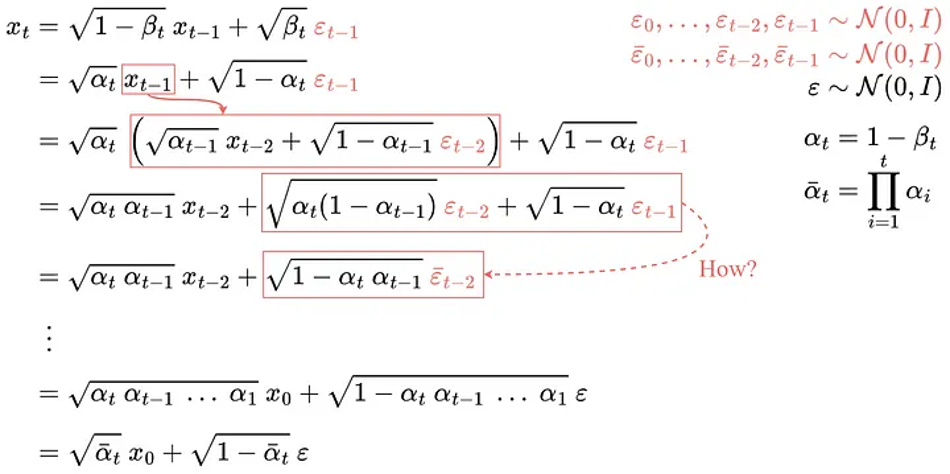
\includegraphics[width=0.7\textwidth]{figs/Q3_2.png}
        \caption{قسمت اول پاسخ بخش ب}
        \label{fig:q3_2}  
    \end{figure}\\
    برای پریدن از خط 4 به 5 در فرمول‌های شکل\ref{fig:q3_2} دقت شود که نویزها باید دارای توزیع گوسی باشند زیرا از این ویژگی که حاصل ترکیب (جمع) دو متغیر گوسی، نیز گوسی می‌شود به صورت زیر در شکل \ref{fig:q3_2_1} استفاده می‌کنیم: (همان راه حل بالا با جزییات بیشتر)
    \begin{figure}[ht]
        \centering
        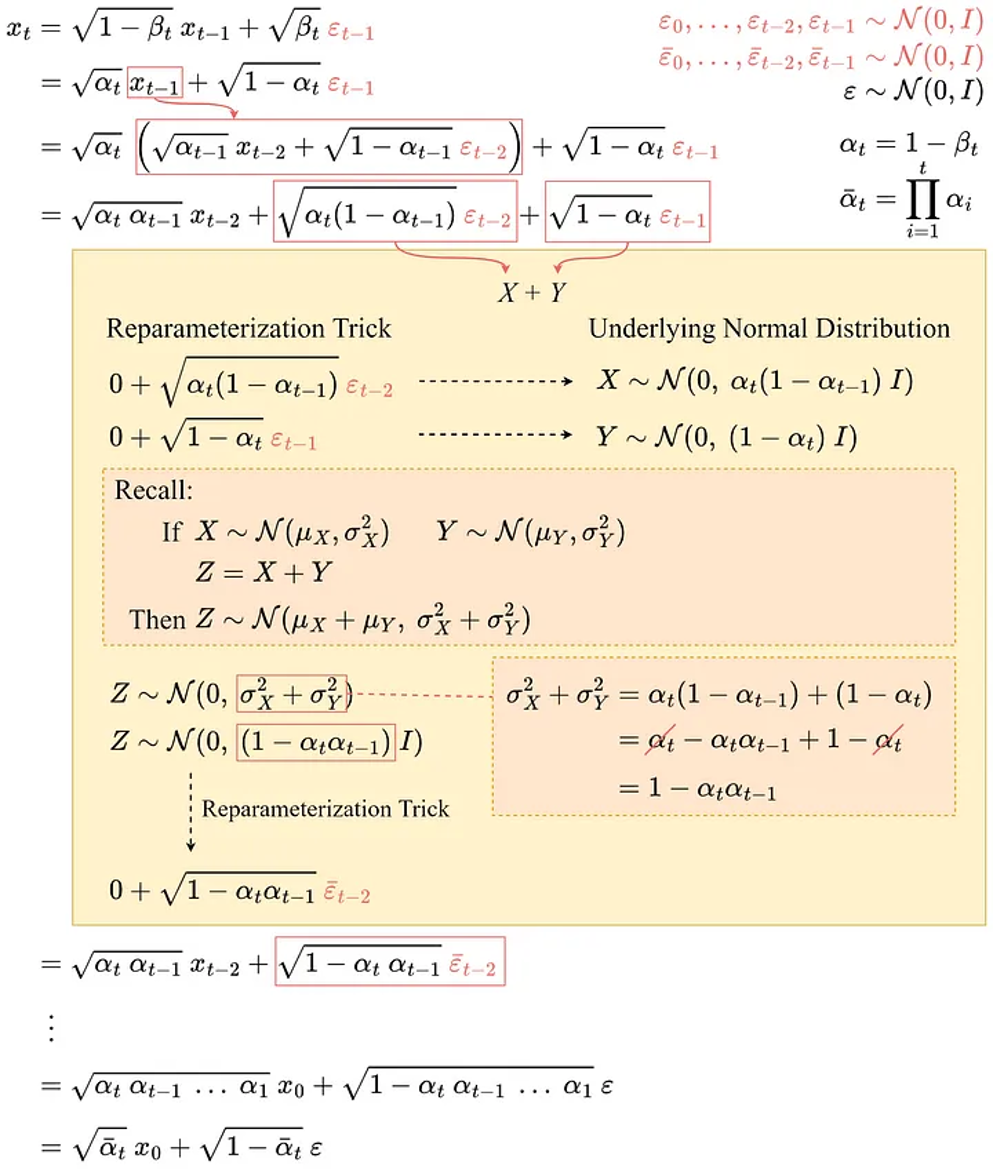
\includegraphics[width=0.7\textwidth]{figs/Q3_2_1.png}
        \caption{قسمت دوم پاسخ بخش ب}
        \label{fig:q3_2_1}  
    \end{figure}\\
    }
    \item با توجه به شکل \ref{fig:q4}  توضیح دهید که چرا به هنگام حذف نویز از داده در فرایند \lr{Reverse Diffusion Process} در هر مرحله نمی‌توانیم به طور مستقیم نویز را حذف کنیم(از $x_{t}$ به $x_{t-1}$ برسیم) و چرا این عمل برایمان غیرقابل حل \LTRfootnote{intractable}می‌باشد؟ (با توجه به شکل \ref{fig:q4} این امر موجب می‌شود تا از روش‌های تخمین تابع مانند شبکه‌های عصبی استفاده کنیم.)
    \begin{figure}[ht]
        \centering
        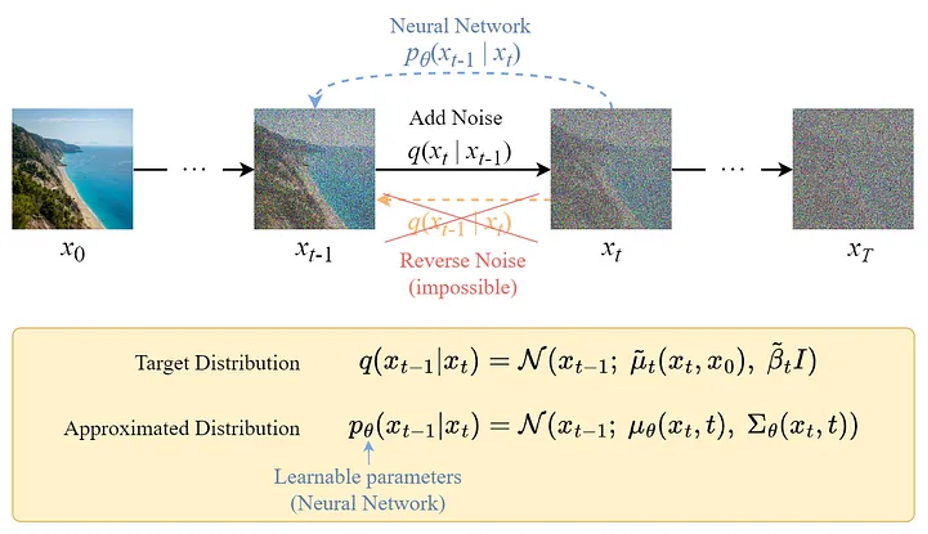
\includegraphics[width=0.85\textwidth]{figs/Q4.png}
        \caption{تابع توزیع تخمین‌زده‌شده توسط شبکه‌ی عصبی}
        \label{fig:q4}  
    \end{figure}

    \textcolor{blue}{
    دلیل اینکه این عمل به طور مستقیم غیرقابل حل (\lr{Intractable}) است، به ماهیت توزیع‌های احتمالی برمی‌گردد. به عبارتی:
    \begin{itemize}
        \item \textbf{ناشناخته بودن توزیع معکوس:} توزیع واقعی فرایند معکوس یک توزیع ساده و مشخص مانند توزیع‌های گوسی نیست. این توزیع به تمام داده‌های آموزشی و مسیر انتشار رو به جلو بستگی دارد و محاسبه آن از نظر محاسباتی غیرممکن است. این یعنی ما نمی‌توانیم فرمولی مستقیم برای حذف نویز بنویسیم.
        \item \textbf{پیچیدگی فرایند:} برای محاسبه دقیق $q(x_{t-1} \mid x_t)$ باید از تمام مسیرهای ممکن به $x_t$ از $x_{t-1}$ نمونه‌برداری کنیم و آن‌ها را به طور کامل در نظر بگیریم، که این کار از نظر محاسباتی بسیار پیچیده است.
    \end{itemize}
    }

    \item تحقیق کنید که چه ویژگی‌هایی از مدل \lr{U-Net} موجب شد که نویسندگان مقاله \lr{DDPM} از آن برای معماری کار خود استفاده کنند؟

    \textcolor{blue}{
    نویسندگان مقاله \lr{DDPM} از معماری \lr{U-Net} به دلیل ویژگی‌های کلیدی آن که کاملاً با وظیفه حذف نویز در این مدل همخوانی دارد، استفاده کردند. مهم‌ترین ویژگی‌های \lr{U-Net} که آن را برای \lr{DDPM} مناسب می‌سازند عبارتند از:
    \begin{itemize}
        \item \textbf{ساختار \lr{Encoder-Decoder}:} مدل \lr{U-Net} از یک مسیر انکودر (\lr{Encoder}) برای فشرده‌سازی تصویر و استخراج ویژگی‌های سطح بالا (مانند شکل‌ها و محتوای کلی) و یک مسیر دیکودر (\lr{Decoder}) برای بازسازی تصویر با جزئیات دقیق استفاده می‌کند. در \lr{DDPM}، انکودر به شبکه عصبی کمک می‌کند تا محتوای کلی تصویر نویزدار ($x_t$) را درک کند و دیکودر با استفاده از این اطلاعات، نویز دقیقاً در هر پیکسل را تخمین بزند.
        \item \textbf{اتصالات میان‌بر (\lr{Skip Connections}):} این ویژگی حیاتی‌ترین جزء \lr{U-Net} برای \lr{DDPM} است. اتصالات میان‌بر، ویژگی‌های سطح پایین (با جزئیات فضایی بالا) را مستقیماً از انکودر به دیکودر در سطوح مشابه وصل می‌کنند. وظیفه اصلی در فرایند معکوس، تخمین نویز در هر پیکسل است. این کار نیاز به حفظ دقیق جزئیات فضایی تصویر دارد. اتصالات میان‌بر باعث می‌شوند که اطلاعات دقیق مکانی که ممکن است در مراحل فشرده‌سازی انکودر از دست برود، به دیکودر منتقل شده و در نتیجه، تخمین نویز با دقت بسیار بالایی انجام شود و تصویر نهایی کیفیت بهتری داشته باشد.
    \end{itemize}
    به طور خلاصه، \lr{U-Net} با ترکیب اطلاعات کلی (معنایی) از طریق انکودر و اطلاعات دقیق مکانی از طریق اتصالات میان‌بر، به بهترین شکل برای وظیفه پیش‌بینی نویز پیکسلی مناسب است، و این دقیقاً همان کاری است که ژنراتور در مدل \lr{DDPM} باید انجام دهد.\\
    }
    \end{enumerate}
    
    \section*{سوالات عملی} 
    \item 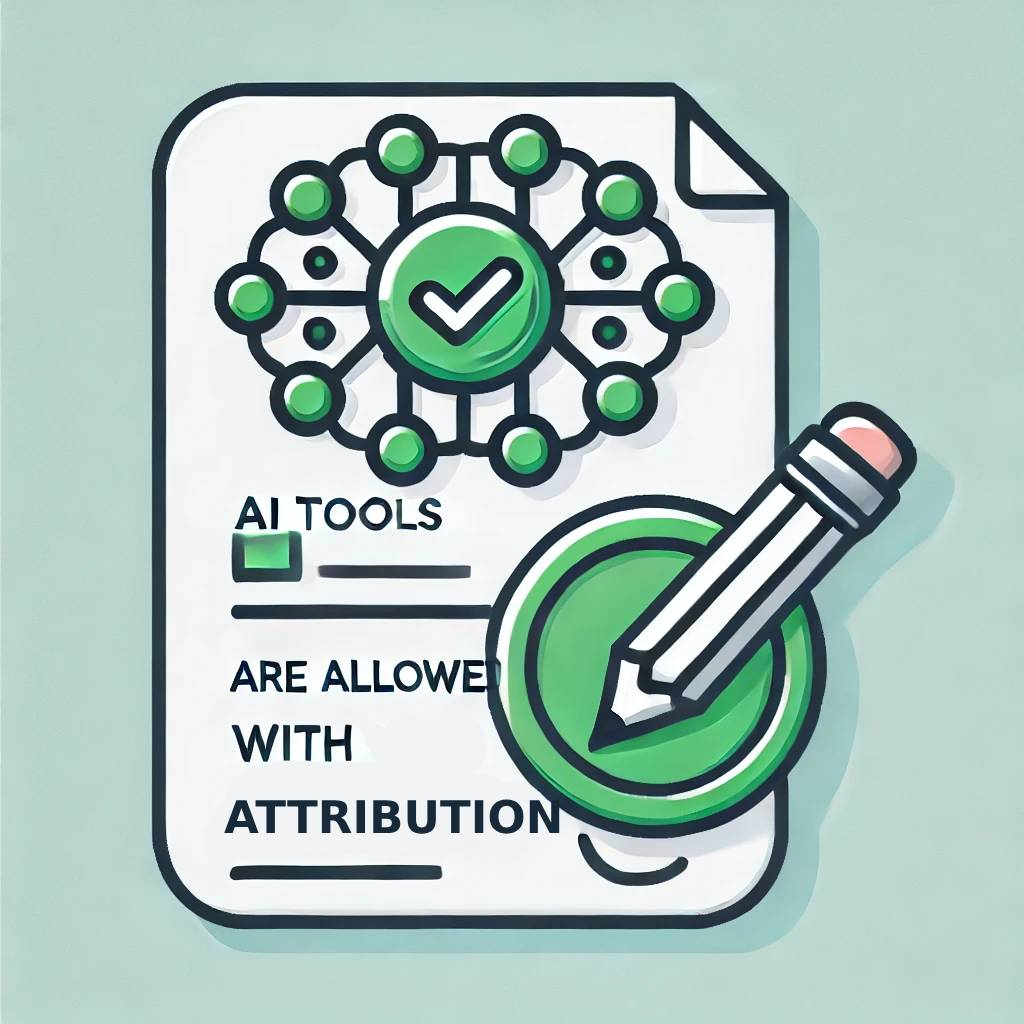
\includegraphics[width=1cm]{figs/Allowed_with_contributino.jpg}
    به این \href{https://github.com/dome272/Diffusion-Models-pytorch}{لینک گیت‌هاب} رفته و به پرسش‌های زیر پاسخ دهید(۲۵ نمره).
    \begin{enumerate}
        \item درباره هدایت بدون دسته‌بند مطالعه کرده و بگویید در کجای کد از آن استفاده شده است؟
        \item شرط در مدل انتشار شرطی به چه شکل اعمال شده است؟ آیا تنها به همین روش می‌توان شرط را اعمال کرد؟ اگر خیر، روش‌های دیگر چیست؟
        \item فرض کنید شرط ما متن باشد و راهنمای بدون طبقه‌بندی را به شکل زیر استفاده کنیم:
        $$
        text_{-}embeddings = text_{-}encoder(["", prompt])
        $$
        کد را بر این اساس تغییر بدهید و بگویید کدام ماژول‌ها تغییر می‌کنند.
        \item  \lr{stable diffusion} چیست؟ کد را براساس آن تغییر دهید و بگویید کدام ماژول‌ها تغییر می‌کنند.

    \end{enumerate}

    \textcolor{blue}{
    \textbf{برای پاسخ این سوال به پوشه \lr{DL\_HW6\_Q4} که از پاسخ آقای پولایی استفاده شده است، مراجعه کنید.}}
    
    \item 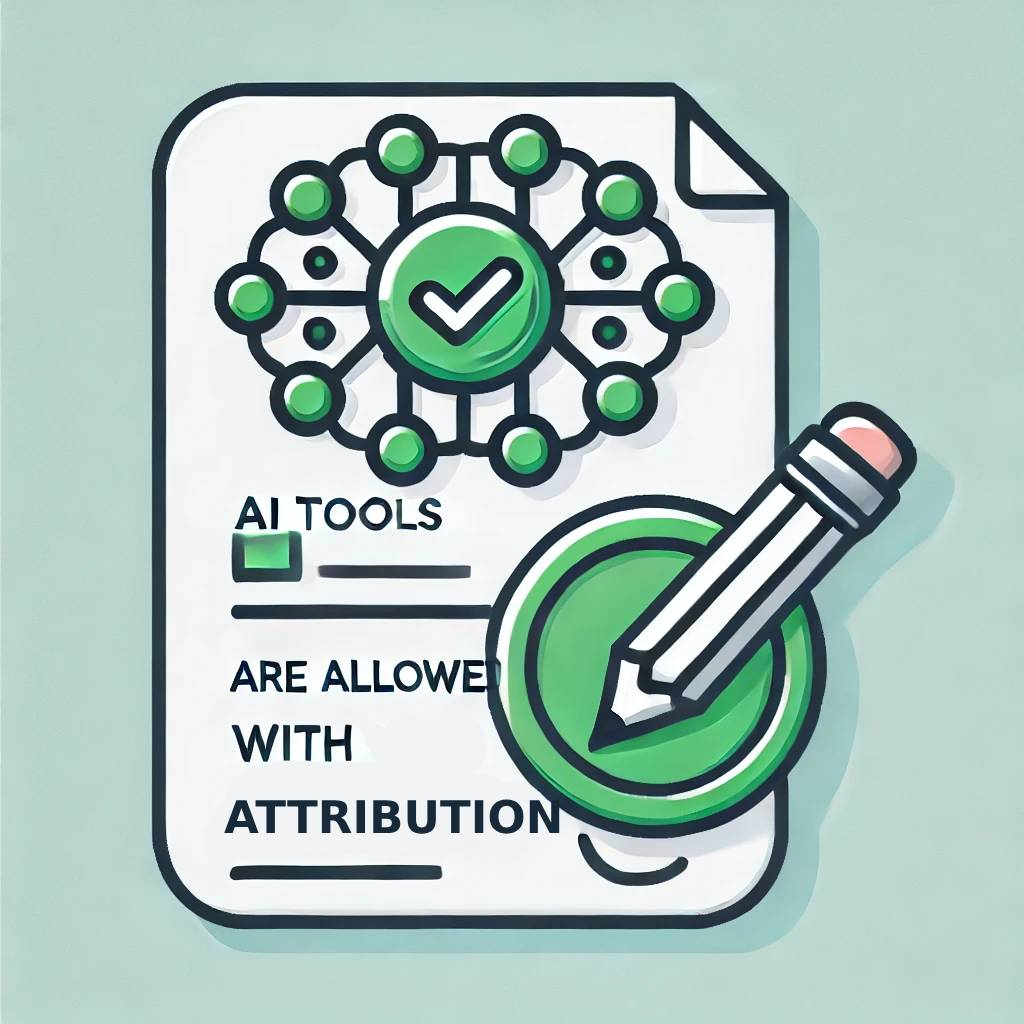
\includegraphics[width=1cm]{figs/Allowed_with_contributino.jpg}
     در این تمرین، شما قرار است دو مدل مولد مهم در یادگیری ماشین را روی مجموعه داده‌ی \lr{MNIST} پیاده‌سازی کنید: خودرمزگذار متغیر (\lr{VAE}) و شبکه مولد تخاصمی (\lr{GAN})(۲۰ نمره).\\
    مدل‌های \lr{VAE} یک متغیر پنهان احتمالاتی را از داده‌های ورودی یاد می‌گیرند، سپس از روی این توزیع نمونه‌برداری کرده و داده‌های جدیدی تولید می‌کنند.\\
    مدل‌های \lr{GAN} از یک شبکه مولد برای تولید تصاویر استفاده می‌کنند که توزیع آن‌ها به توزیع داده‌های واقعی نزدیک است.\\
   نوتبوک \lr{GAN-VAE.ipynb} حاوی کدهایی است که برخی بخش‌های آن با برچسب \lr{TODO} مشخص شده‌اند. شما باید این بخش‌ها را با دقت تکمیل کنید تا مدل‌ها به درستی پیاده‌سازی شوند.\\
    پیشنهاد می‌شود پیش از نوشتن کد، تمامی توضیحات و سلول‌ها را به‌دقت مطالعه کنید تا درک کاملی از ساختار مدل‌ها و نحوه پیاده‌سازی آن‌ها داشته باشید.

    \textcolor{blue}{
    \textbf{برای پاسخ این سوال به نوتبوک \lr{GAN-VAE\_ans.ipynb}} مراجعه کنید.
    }

     \item 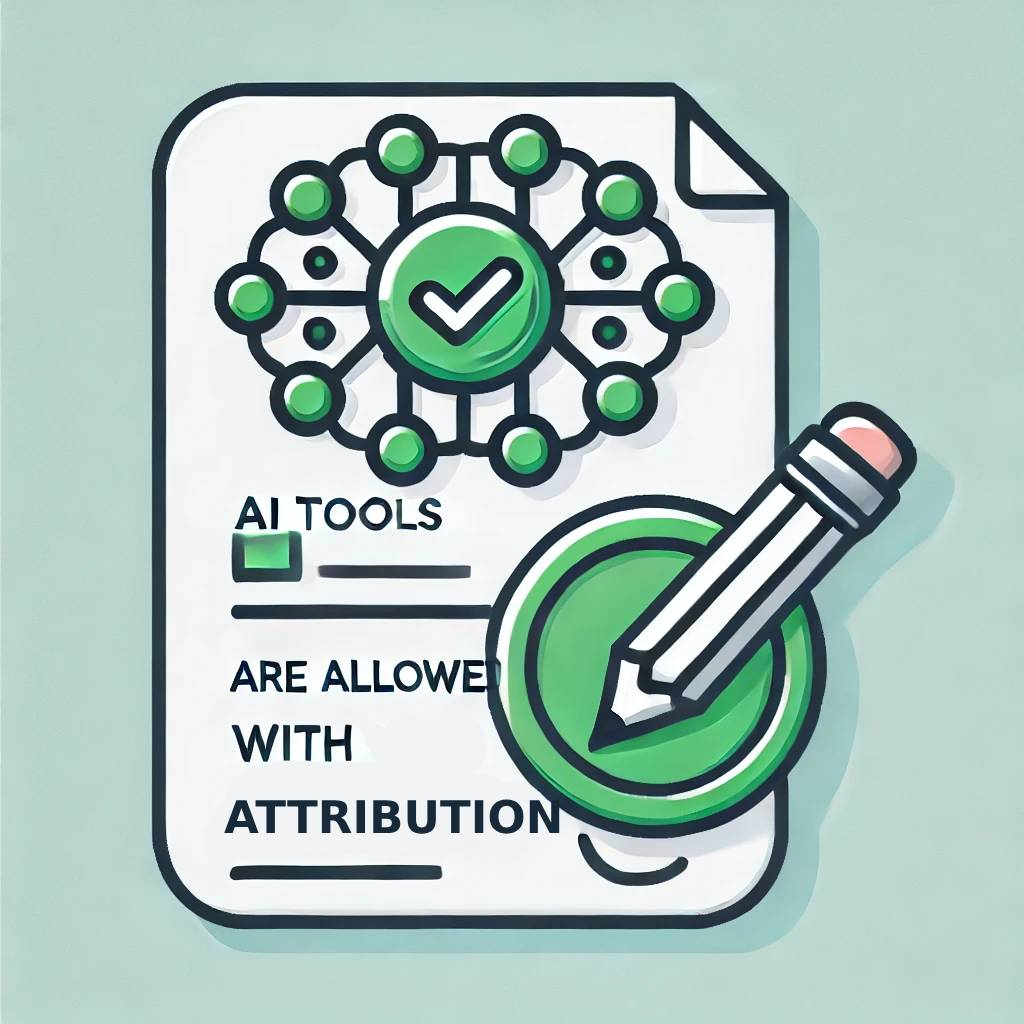
\includegraphics[width=1cm]{figs/Allowed_with_contributino.jpg}
     در این تمرین، هدف شما پیاده‌سازی یک مدل احتمالی انتشار نویز است. برای درک بهتر مفاهیم، توصیه می‌شود مقاله اصلی مربوط به \href{https://arxiv.org/pdf/2006.11239}{\lr{DDPM}} را مطالعه کنید(۲۰ نمره).

    شما باید نوتبوک \lr{DDPM.ipynb} را تکمیل کرده و تمام سلول‌های آن را اجرا کنید. بخش‌هایی که نیاز به تکمیل دارند، با برچسب \lr{TODO} در داخل بلوک‌های کد مشخص شده‌اند.\\
    پیش از شروع به نوشتن کد، تمام توضیحات متنی و کدهای داده‌شده را با دقت بخوانید.\\
    این نوت‌بوک با استفاده از محیط‌های رایگان \lr{Google Colab} و \lr{Kaggle} آزمایش شده است؛ می‌توانید از این پلتفرم‌ها برای اجرای کدهای خود استفاده کنید.\\
    اطمینان حاصل کنید که تمامی سلول‌ها بدون خطا اجرا می‌شوند و عملکرد مورد انتظار را ارائه می‌دهند.\\

    \textcolor{blue}{
    \textbf{برای پاسخ این سوال به نوتبوک \lr{DDPM\_ans.ipynb}} مراجعه کنید.
    }

\end{enumerate}



\end{document}


